% UI contribution for M5: Shahmeer (AI-assisted; reviewed by Shahmeer).
The M4 Flask interface now runs on the knowledge graph
(Figure~\ref{fig:architecture}). Users still search disclosures by ticker,
dimension and date, view source evidence, create disclosures, batch-edit
weights, delete entries and view dated portfolios, but they never write SPARQL.
At startup the integrated factory opens one shared graph, loads the ontology into
its own named graph and attaches both validators. The graph repositories keep the
M4 function signatures, result keys and error classes, so each route needed only
a data-access swap. Routes hold neither SQL nor SPARQL; the business layer still checks
dates, fractions, duplicate categories and empty forms.

Every write is staged on a candidate graph and published as one delta only after
validation. Rejected edits keep the user's input and show a plain message, and the business
layer translates validator messages such as duplicate snapshots, dimension
mismatches and unknown references. All 26 M4 route tests were rerun
unchanged against a fresh validated graph, and every rejection left the complete
quad set identical; with three new graph-specific tests the suite reaches 189
passing tests. A script rebuilds a throwaway graph and recaptures the eleven screenshots,
including the six write and rejection cases.

\paragraph{Evaluation and limits.}
A two-entry Complete snapshot (0.3, 0.7) rejects an edit to (0.1, 0.7), but
accepts the atomic batch (0.4, 0.6). Deleting a Partial entry succeeds; deleting
its final entry fails. Rejections preserve all quads, including the TBox, rather
than merely producing an error message. SQL parity verifies representation on
the seed, not real provider facts. The 0.005 tolerance is provisional, not measured
rounding error; synthetic captures exercise provenance, not independent financial
verification. One writable process is supported; no scalability or performance
claim follows from this demonstration.

% Architecture figure (full width):
% \begin{figure*}[t]
%   \centering
%   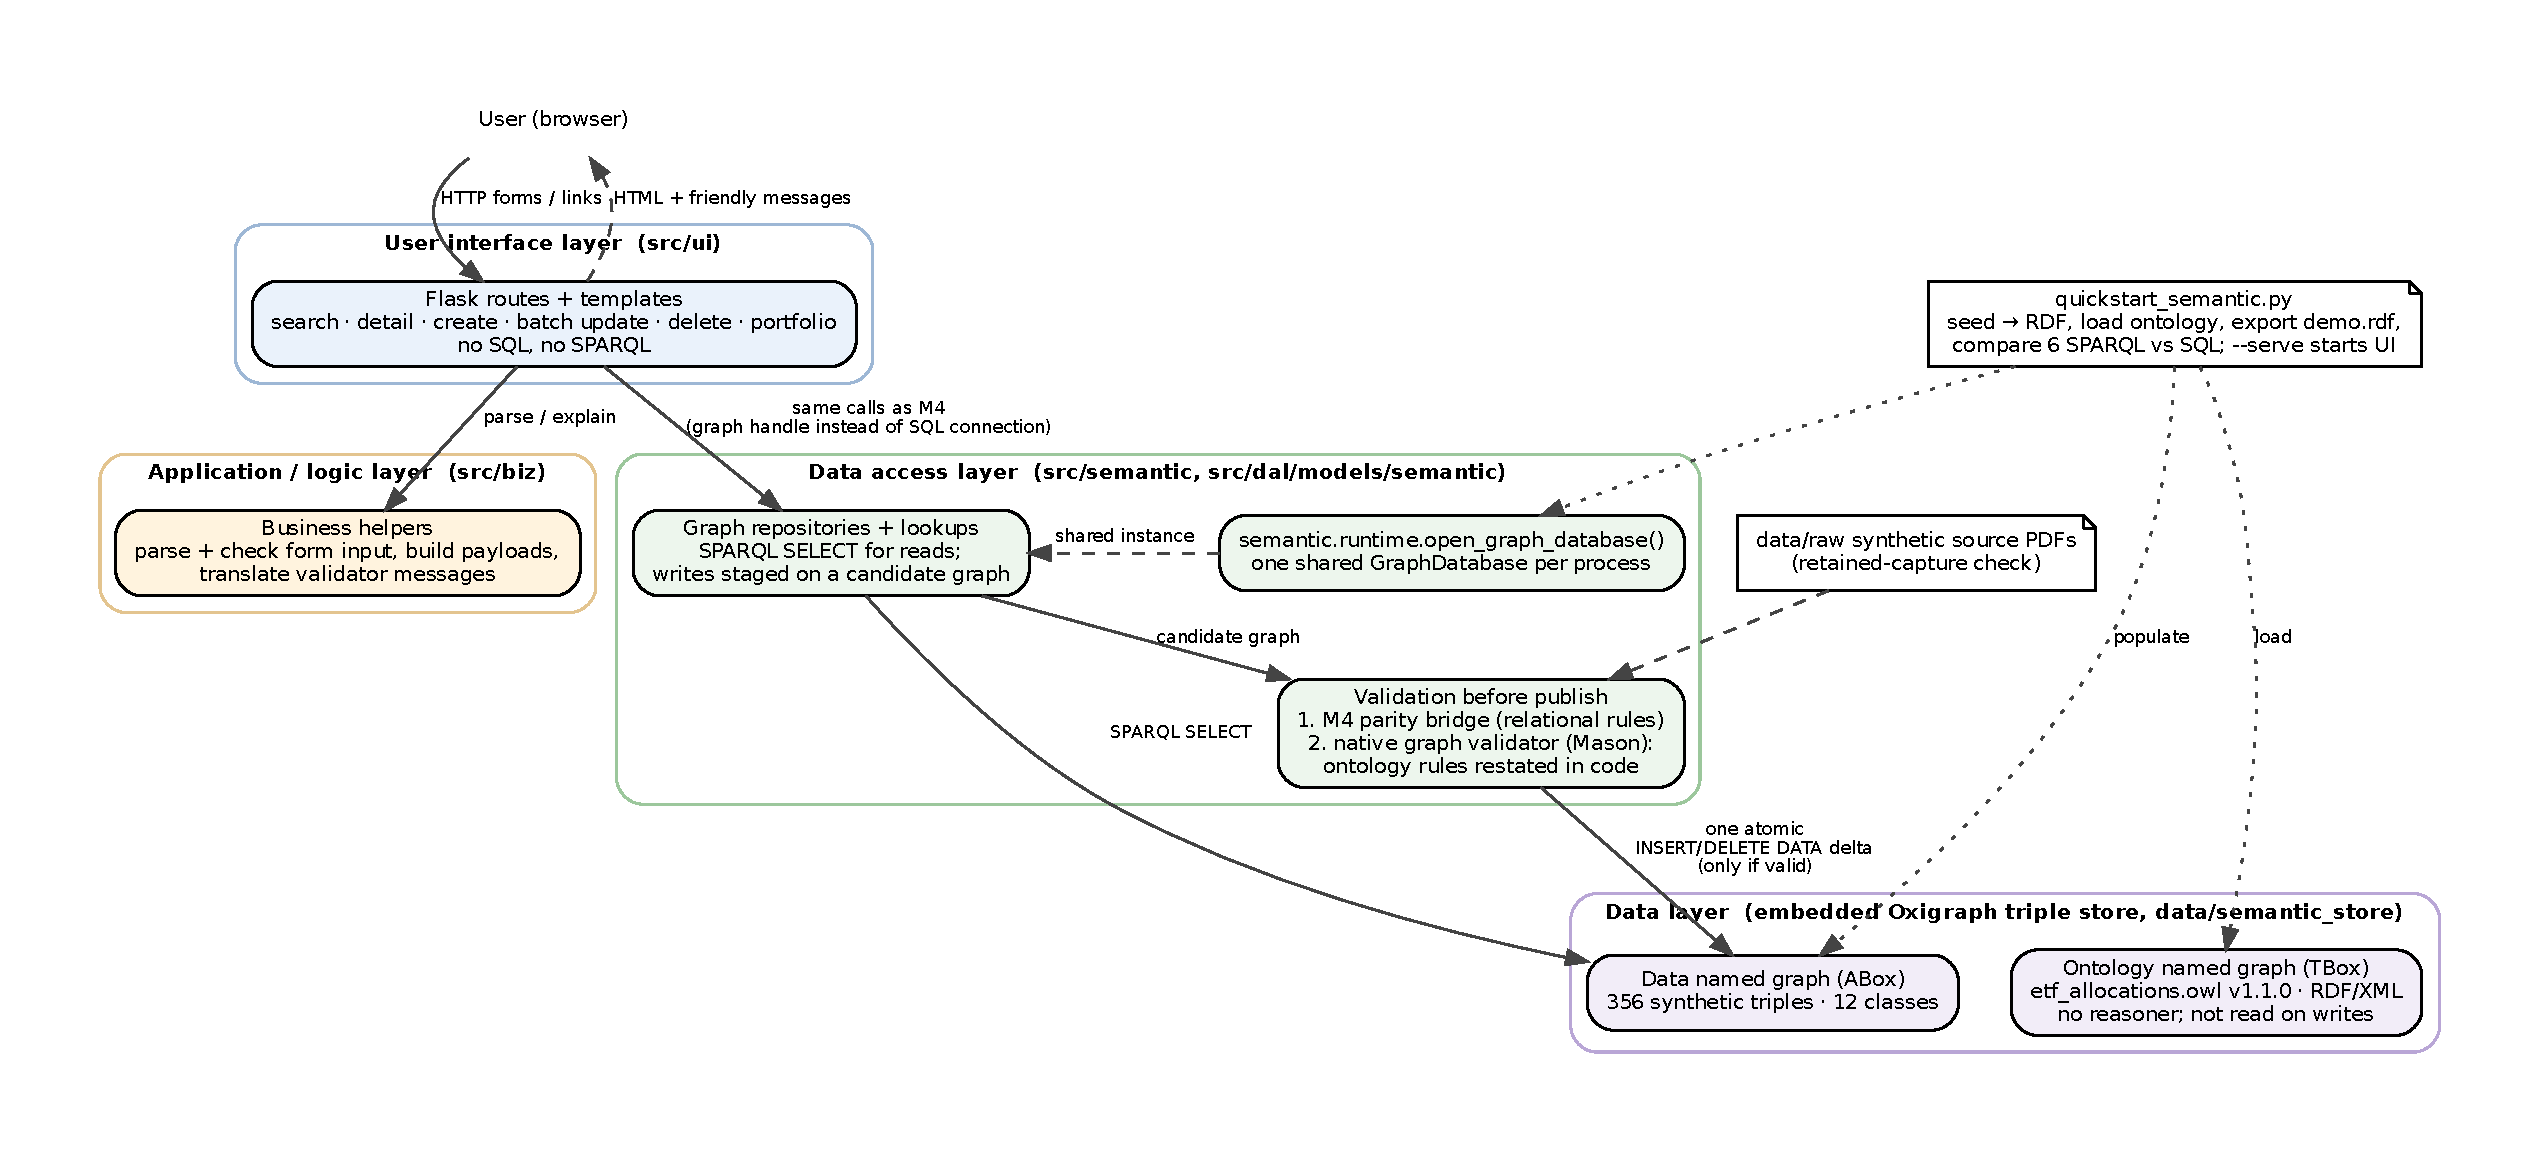
\includegraphics[width=\textwidth]{figures/system_architecture_m5.pdf}
%   \caption{M5 layers: Flask UI, business helpers, graph data access with
%   validation before publish, and the embedded Oxigraph store holding separate
%   ontology and data named graphs.}
%   \label{fig:architecture}
% \end{figure*}
